\documentclass[11pt]{article}
\usepackage{lipsum}
\usepackage[letterpaper, landscape, twocolumn, left=0.5in, right=0.5in, top=1.25in, bottom=0.75in, headheight=0.6in]{geometry} % controls page layout
\usepackage{fancyhdr} % controls headers and footers
\usepackage{lastpage} % enables # of ##
\usepackage{graphicx} % graphics
\usepackage{grffile} % enables multiple periods in file name of \includegraphics
\usepackage{amsmath}  % extended mathematics
\usepackage{booktabs} % book-quality tables
\usepackage{units}    % non-stacked fractions and better unit spacing
\usepackage[T1]{fontenc} % 8-bit encoding of fonts (glyphs are a part of fonts)

\fancypagestyle{title}{ % defining header style for the first page
  \fancyhead[C,R]{}
  \fancyhead[L]{\begin{tabular}{ll}
  \raisebox{-.47\height}{
\includegraphics[height=0.75in, trim=0 -0.1in 0 0]{visuals/SCE_logo}} &
  \textsc{\textbf{\Huge Customer Report for: <CustomerID>}}
  \end{tabular}}
  \fancyfoot[L]{\today}
  \fancyfoot[C]{}
  \fancyfoot[R]{\thepage/\pageref{LastPage}}
}

\fancypagestyle{energy}{ % header style for energy charges
  \fancyhead[L]{\textsc{\textbf{\Huge Energy Charges}}}
  \fancyhead[C]{}
  \fancyhead[R]{\textsc{\textbf{\Huge <CustomerID>}}}
  \fancyfoot[L]{\today}
  \fancyfoot[C]{}
  \fancyfoot[R]{\thepage/\pageref{LastPage}}
}

\fancypagestyle{demand}{ % header style for demand charges
  \fancyhead[L]{\textsc{\textbf{\Huge Demand Charges}}}
  \fancyhead[C]{}
  \fancyhead[R]{\textsc{\textbf{\Huge <CustomerID>}}}
  \fancyfoot[L]{\today}
  \fancyfoot[C]{}
  \fancyfoot[R]{\thepage/\pageref{LastPage}}
}

\renewcommand{\headrulewidth}{0.4pt}
\renewcommand{\footrulewidth}{0.4pt}

\begin{document}
\pagestyle{title}
This report summarizes your electricity charges relative to your usage patterns. It also compares your usage patterns relative to those of others in your ``peer group'', those with the same North American Industry (NAICS) code and subscribed to the same time of use rate (TOU). It is provided to you for your information and as a backdrop for the conversation with Southern California Edison (SCE) to find opportunities for savings.

The analysis is performed by back-casting your last year's consumption to the rates currently in effect. As such, it is a forecast of your future payments, not an accurate replica of your earlier ones.

\vspace{3ex}
\textbf{\Large Components of the Bill}
\vspace{1ex}

The electric bill has three main components: facility charges, energy charges, and demand charges. The makeup of these charges for the year and by month are shown in Figures~\ref{fig:pie} and \ref{fig:bars}, respectively.
\begin{figure}[!h]
\centering
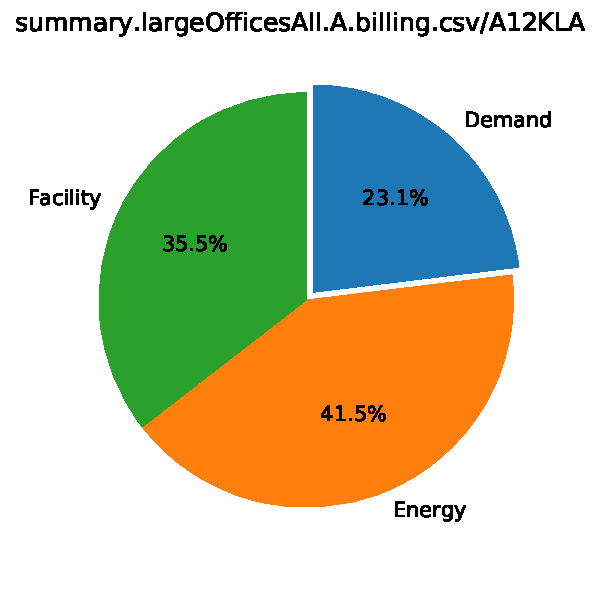
\includegraphics[height=3in, page=1, trim=0in 0.45in 0in 0.45in, clip]{visuals/largeOfficesAll.A.piecharts.pdf}
\caption{Makeup of annual charges}
\label{fig:pie}
\end{figure}

\begin{figure}[!h]
\centering
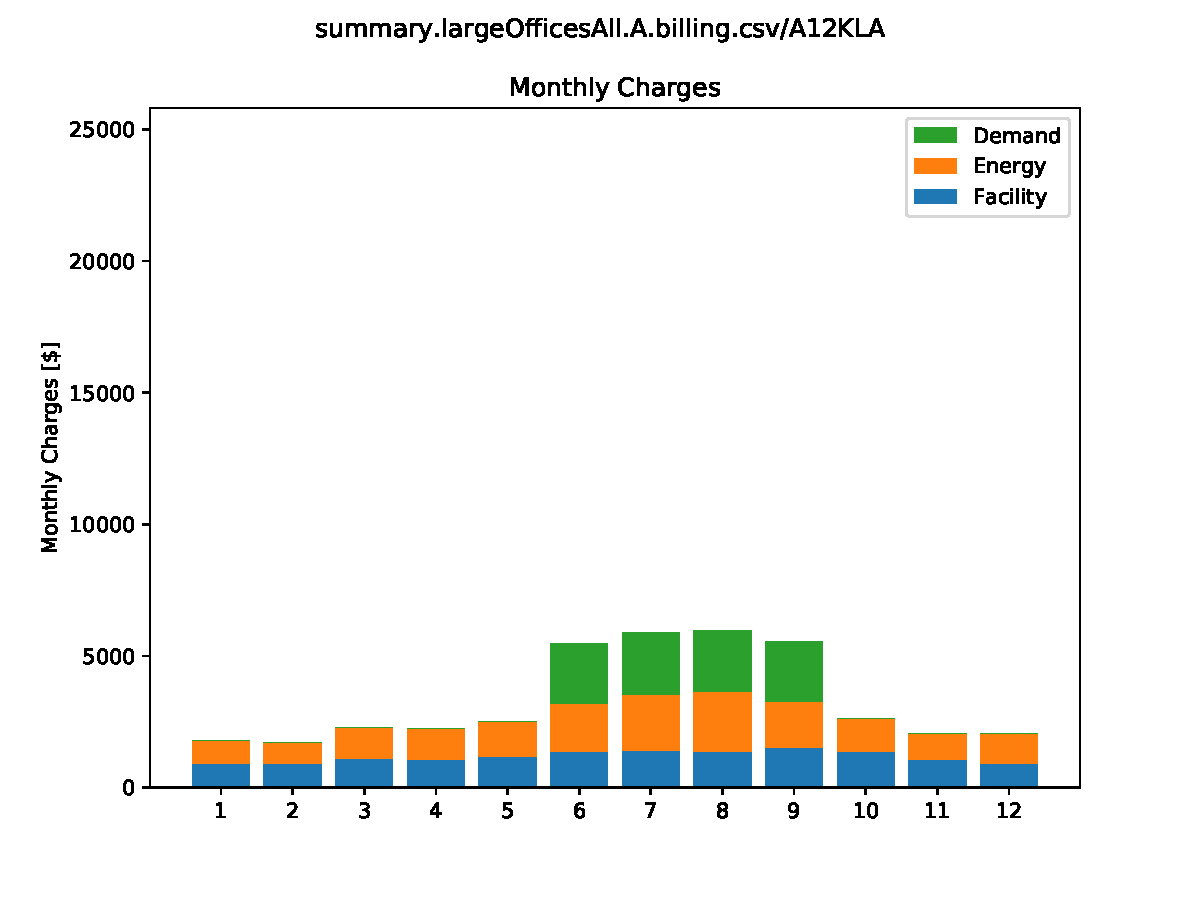
\includegraphics[width=\columnwidth, page=1, trim=0in 0.45in 0in 0.45in, clip]{visuals/largeOfficesAll.A.boxplots.pdf}
\caption{Makeup of monthly charges}
\label{fig:bars}
\end{figure}

Note that the demand charges are collected only in the four summer months, yet they account for <dmndpc> of the total annual bill. The expected annual charges by bill component are summarized in Table~\ref{tab:annual}.

\begin{table}[th!]
  \centering
  \caption{Components of annual electric bill}
  \vspace{1.5ex}
  \label{tab:energy}
  \begin{tabular}{ll}
    Bill component & Amount [\$] \\
    \midrule
    Facility & <facility> \\
    Energy & <energy> \\
    Demand & <demand> \\
    \midrule
    Total & <total>
  \end{tabular}
\end{table}
\clearpage

\newgeometry{twocolumn, left=0.5in, right=0.5in, top=0.75in, bottom=0.75in, headheight=0.1in}
\pagestyle{energy}

\begin{figure}[!h]
\centering
\includegraphics[width=\columnwidth, page=1, trim=0in 0.45in 0in 0.45in, clip]{visuals/largeOfficesAll.A.heatmaps.pdf}
\caption{Normalized consumption for <CustomerID>}
\label{fig:heatmap}
\end{figure}

\begin{figure}[!h]
\centering
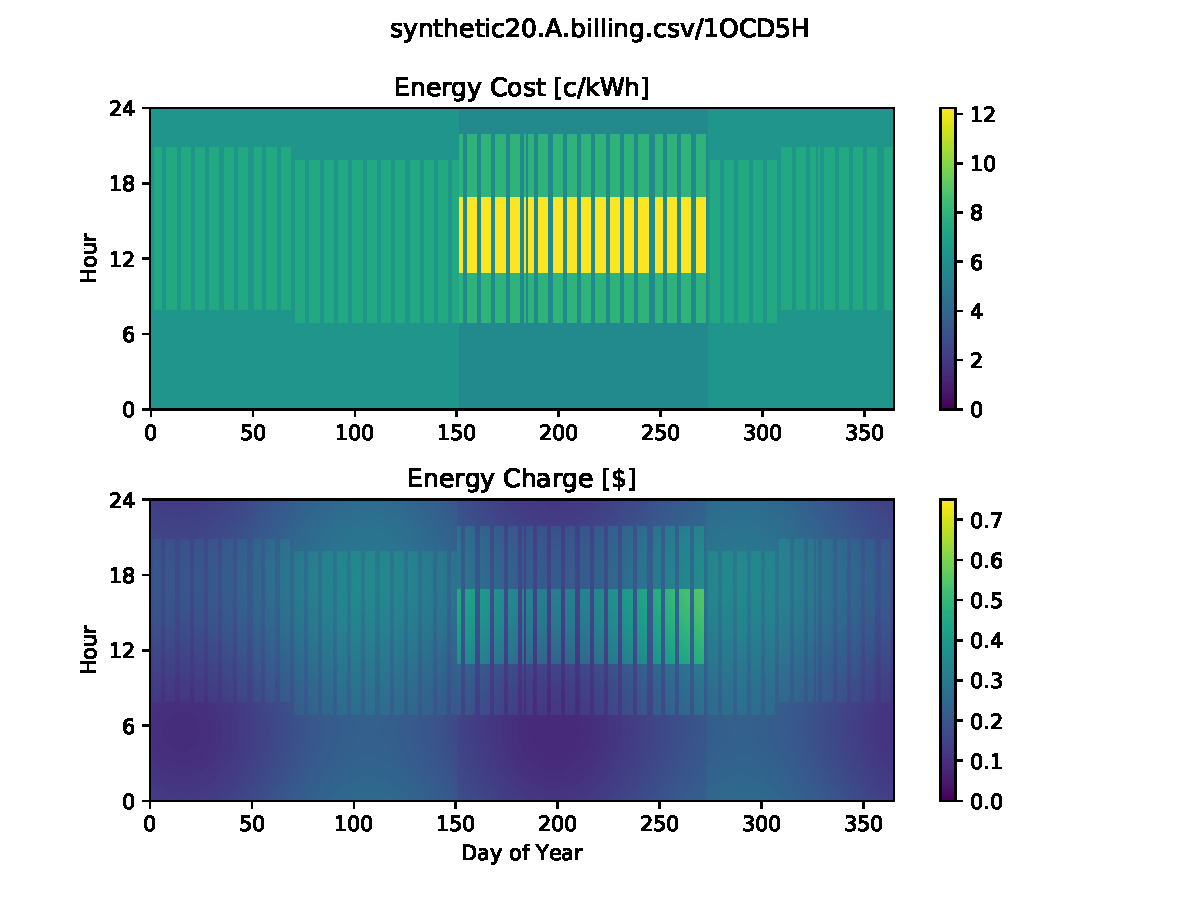
\includegraphics[width=\columnwidth, page=1, trim=0in 3in 0in 0.45in, clip]{visuals/synthetic20.A.billing.Heatmaps.pdf}
\caption{Energy price on <RateCode>}
\label{fig:toumap}
\end{figure}

\lipsum[1][1-7]

\begin{table}[th!]
  \centering
  \caption{Components of annual electric bill}
  \vspace{1.5ex}
  \label{tab:annual}
  \begin{tabular}{llll}
    Month & Avg price [\$] & Month & Avg price [\$] \\
    \midrule
    Jan & <EnAvg01> & Jul & <EnAvg07> \\
    Feb & <EnAvg02> & Aug & <EnAvg08> \\
    Mar & <EnAvg03> & Sep & <EnAvg09> \\
    Apr & <EnAvg04> & Oct & <EnAvg10> \\
    Jun & <EnAvg06> & Nov & <EnAvg11> \\
    May & <EnAvg05> & Dec & <EnAvg12> \\
    \midrule
    Annual average & <EnAvgAnnual>
  \end{tabular}
\end{table}

\vspace{3ex}
\textbf{\Large Peer performance}
\vspace{1ex}

\lipsum[1][1-7]

\begin{figure}[!h]
\centering
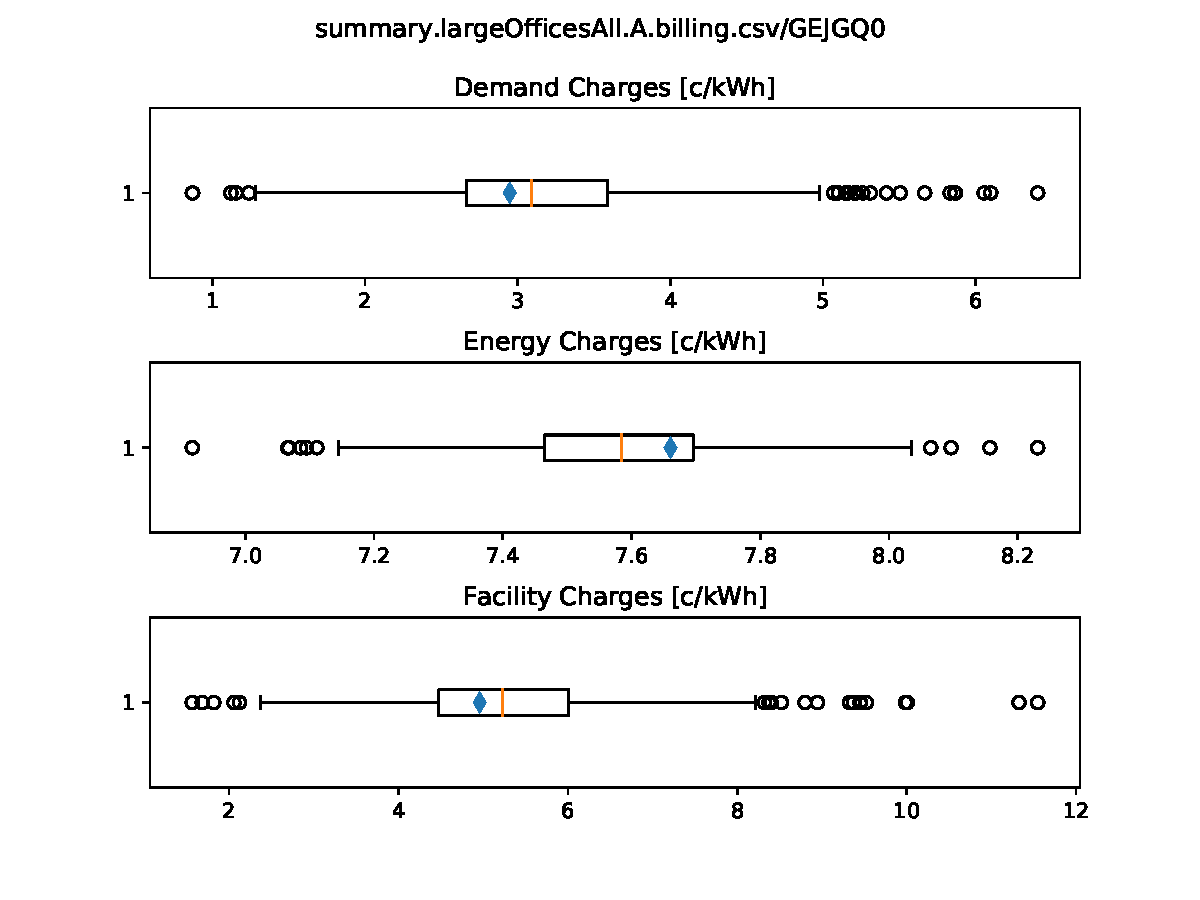
\includegraphics[width=\columnwidth, page=1, trim=0in 2.1in 0in 2.1in, clip]{visuals/largeOfficesAll.A.whiskercharts.pdf}
\caption{Average annual energy price for <CustomerID> compared to peers}
\label{fig:PeerCompEn}
\end{figure}

\clearpage

\newgeometry{twocolumn, left=0.5in, right=0.5in, top=0.75in, bottom=0.75in, headheight=0.1in}
\pagestyle{demand}
\lipsum[1][1-7]

\begin{figure}[!h]
\centering
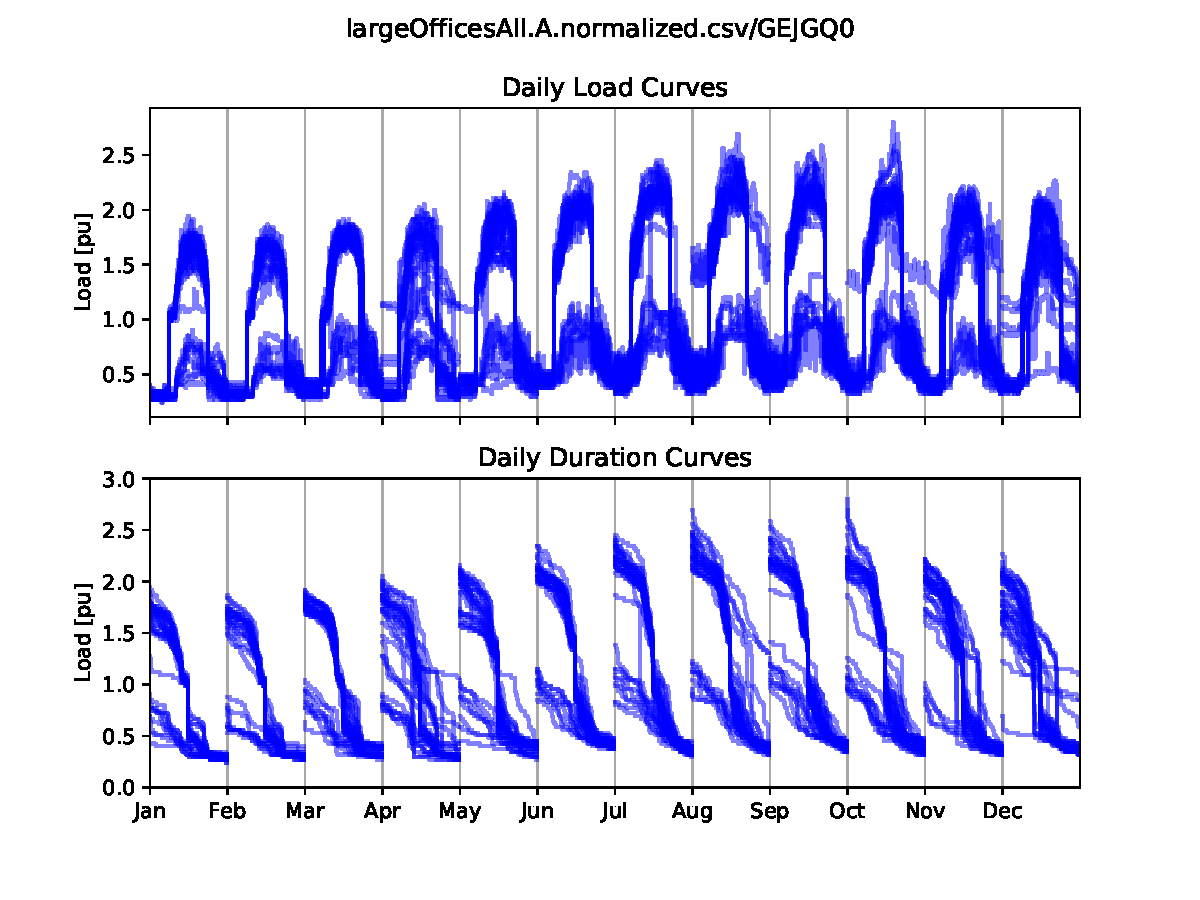
\includegraphics[width=\columnwidth, page=1, trim=0in 0.45in 0in 0.45in, clip]{visuals/largeOfficesAll.A.duration.monthly.test.pdf}
\caption{Normalized consumption for <CustomerID>}
\label{fig:duration}
\end{figure}

\lipsum[1][1-7]

\begin{table}[th!]
  \centering
  \caption{Monthly Demand Charges}
  \vspace{1.5ex}
  \label{tab:demand}
  \begin{tabular}{llll}
    Month & Avg price [\$] & Month & Avg price [\$] \\
    \midrule
    Jan & <EnAvg01> & Jul & <EnAvg07> \\
    Feb & <EnAvg02> & Aug & <EnAvg08> \\
    Mar & <EnAvg03> & Sep & <EnAvg09> \\
    Apr & <EnAvg04> & Oct & <EnAvg10> \\
    Jun & <EnAvg06> & Nov & <EnAvg11> \\
    May & <EnAvg05> & Dec & <EnAvg12> \\
    \midrule
    Annual average & <DmndAvgAnnual>
  \end{tabular}
\end{table}

\vspace{3ex}
\textbf{\Large Peer performance}
\vspace{1ex}

\lipsum[1][1-7]

\begin{figure}[!h]
\centering
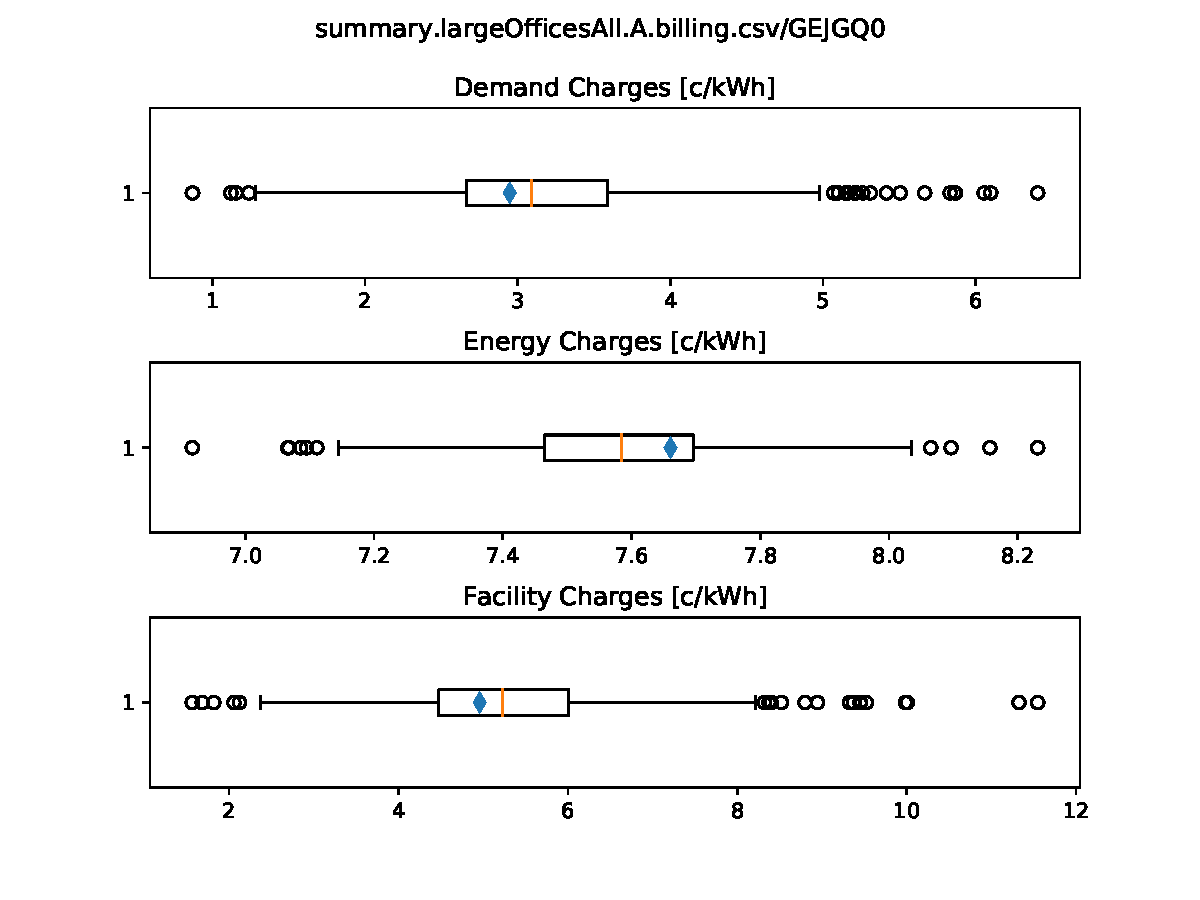
\includegraphics[width=\columnwidth, page=1, trim=0in 3.8in 0in 0.5in, clip]{visuals/largeOfficesAll.A.whiskercharts.pdf}
\caption{Average annual demand price for <CustomerID> compared to peers}
\label{fig:PeerCompDmnd}
\end{figure}

\end{document}
